\subsubsection{Core structure}\label{sec:core}
\begin{figure}[ht] 
	\centering
	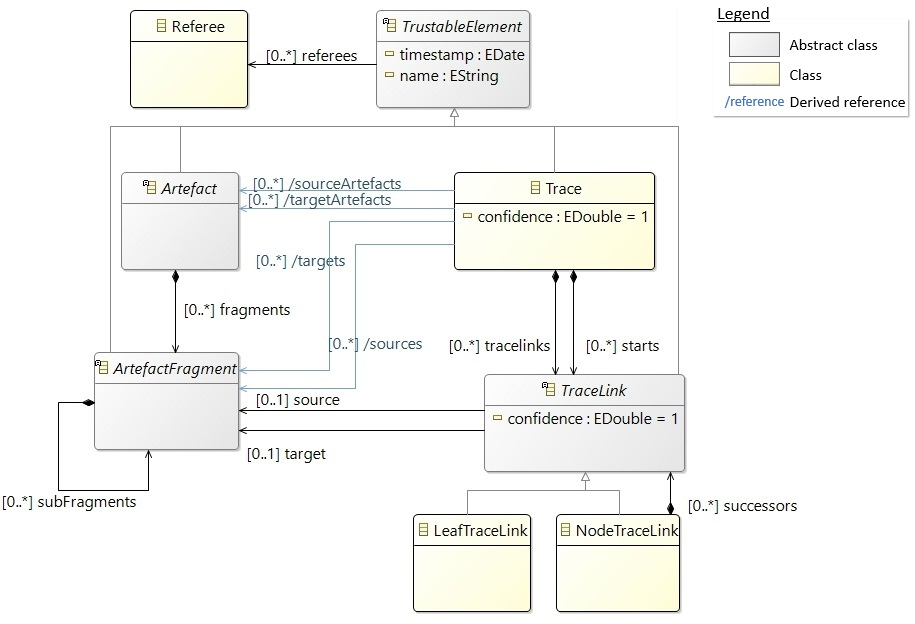
\includegraphics[width=.85\linewidth]{images/core.jpg}
	\caption{Core structure of Tracea metamodel}
	\label{fig:mm-core}
\end{figure}

The core of traceability is to arbitrarily bind artefacts of a system(s) with each others. A trace may have one or many sources and ends with one or many targets. The connection among the artefacts in a trace is expressed as the combination of atomic trace links representing direct connections between a number of fragments of each involved artefact.

Fig. \ref{fig:mm-core} shows an excerpt of Tracea metamodel. This excerpt describes the core structure of traces. It describes the composition scheme of its links (bottom right corner), offers an interface for the decomposition of artefacts into fragments (left side), and allows to record information related to the authorities potentially accountable for its constituents (top class).
%Tracing may refer to \textit{i)} the link between two entities of specific kind: a simple direct link; \textit{ii)} a succession of links from an arbitrary artefact to another; or \textit{iii)} a set of \textit{complex intertwined links}.

\paragraph{Classes}
\begin{itemize}
    \item A \texttt{Trace} is a composition of \texttt{TraceLinks}. It references the source of trace links (\textit{starts} reference) as well as the trace links involved to access the different artefacts (\textit{tracelinks} reference). 
    A trace also references to source and target artefacts and fragments. These references are derived from the \texttt{TraceLinks}.
    \item A \texttt{TraceLink} is the fundamental structure to build the trace sequences and branches. It is a direct connection between two elements of the system (\textit{i.e.,} \texttt{ArtefactFragments}). A \texttt{TraceLink} has one source fragment and one target fragment. It is also the abstract node of a tree of \texttt{TraceLinkNode} and A \texttt{TraceLinkLeaf} refers to a list of successors being part of the linkage of the trace. This class is abstract and is refined into \texttt{NodeTraceLink} and \texttt{LeafTraceLink} following the Composite design pattern.
    \item A \texttt{NodeTraceLink} is a node in a tree like \texttt{TraceLink}. It references successor links.
    \item A \texttt{LeafTraceLink} is a leaf in a tree-like \texttt{TraceLink}. It has no successor link reference.
    \item An \texttt{Artefact} is an abstract representation of an element of the traced system. An artefact represent a text document, a class diagram, or any other kind of document. (See Section~\ref{sec:granularity})
    \item A \texttt{ArtefactFragment} is a part of an Artefact. It can be further decomposed into sub fragments for finer granularity. (See Section~\ref{sec:granularity})
    \item A \texttt{TrustableElement}: Is an abstract class representing elements that have am identifier (name) and a timestamp for timed traceability consideration. It also references \texttt{Referees} to its specializations (\textit{i.e.,} \texttt{Trace}, \texttt{TraceLink}, \texttt{Artefact}, \texttt{ArtefactFragment}, \texttt{Evidence} - see Section \ref{sec:integrity} for details).
    \item A \texttt{Referee} is an actor accountable for a \texttt{TrusteableElement} (See Section~\ref{sec:integrity})
\end{itemize} 

\pagebreak
\paragraph{Well-formedness rules}
Well-formedness rules are expressed as OCL constraints. 
Rules in Figure \ref{fig:ocl-core} ensure that the inclusion of starters in the list of links a trace have, and the derivation of derived references related to source and target artefacts and fragments. 
\begin{figure*}[h]
\centering 
\rule{0.9\linewidth}{1pt}
\vspace{-0.2truecm}
\small
\begin{ocl}[0.85\linewidth]

\vspace{0.3truecm}\OCLcontext~Trace \OCLinv ~starters: \\ \verb+     +\OCLself.tracelinks \OCLarrow includesAll(\OCLself.starts)  

\vspace{0.3truecm}\OCLcontext~Trace \OCLinv ~derivedSources: \\ \verb+     +\OCLself.tracelinks\OCLarrow collect(source) 
\\ \verb+     +\OCLarrow includesAll(\OCLself.sources)   

\vspace{0.3truecm}\OCLcontext~Trace \OCLinv ~derivedTargets: \\ \verb+     +\OCLself.tracelinks \OCLarrow collect(target) 
\\ \verb+     +\OCLarrow includesAll(\OCLself.targets)   

\vspace{0.3truecm}\OCLcontext~Trace \OCLinv ~derivedSourceArtefacts: \\ \verb+     +\OCLself.tracelinks \OCLarrow collect(source)  
\\ \verb+     +\OCLarrow includesAll(\OCLself.sourceArtefacts.fragments)   

\vspace{0.3truecm}\OCLcontext~Trace \OCLinv ~derivedTargetArtefacts: \\ \verb+     +\OCLself.tracelinks \OCLarrow collect(target)  
\\ \verb+     +\OCLarrow includesAll(\OCLself.targetArtefacts.fragments)   

\end{ocl}

\vspace{0.4truecm}
\rule{0.9\linewidth}{1pt}
\vspace{-0.2truecm}

\caption{OCL constraints over elements of the core package.}
\label{fig:ocl-core}
\vspace{-0.6truecm}
\end{figure*}

\paragraph{Illustrative example}
\begin{figure}[h] 
	\centering
	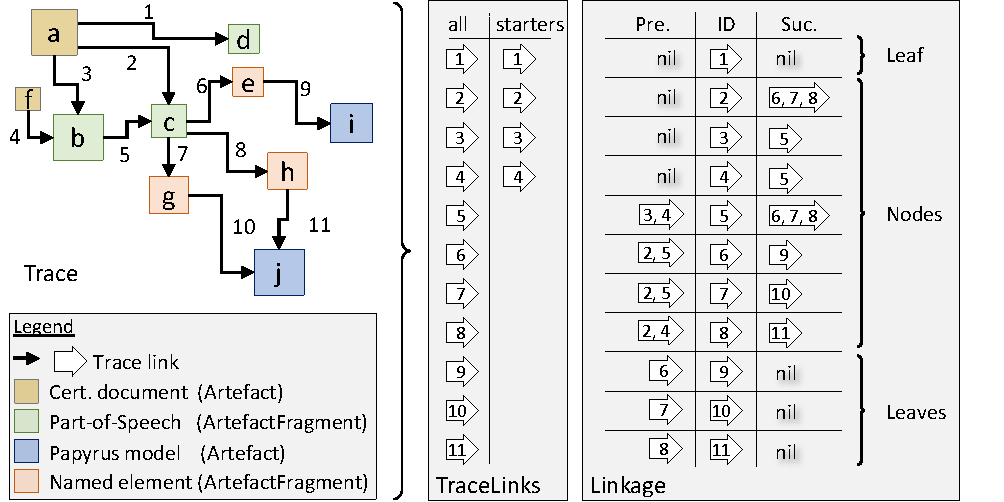
\includegraphics[width=.85\linewidth]{images/core-re}
	\caption{Structure of a transclusion trace. }
	\label{fig:mm-core-instance}
\end{figure}
The core section of the metamodel aims at representing the structure of the linkage between the artefacts that are part of a trace. 
In our example, a trace sequentially links the PoSs in certification documents to their corresponding entities in design models. 
In simple words, a document contains Parts-of-Speech (PoSs) where each PoS is associated to a number of model elements, themselves contained in one or more models. These directions are \texttt{TraceLinks}. Figure \ref{fig:mm-core-instance} shows a diagrammatic perspective of the structure of a transclusion. The example transclusion trace relates the PoS (b, c, and d) of documents (a and f) to the \texttt{NamedElements} (i and j) of three Papyrus models (e, g, h). 
We see on the right side that some \texttt{TraceLinks} have successors, they are \texttt{TraceLinkNode}s; when they do not they are \texttt{TraceLinkLeaf}s. 

When represented as instances of the Tracea metamodel, a certification document is an Artefact, a section of a document is an \texttt{ArtefactFragment}. A PoS is a fragment as well. On the model side, models are \texttt{Artefacts}. Packages, classes, and named elements are \texttt{ArtefactFragments}. We will develop on relationship types in Section \ref{sec:relationshiptype}. 


%Next:  G R A N U L A R I T Y